\chapter{Plasma Overview}
\label{ch:plasma_overview}

Plasma is a fundamental state of matter, along with solid, liquid, and gas. They have a similar characteristics to gases, in that they are compressible and expand to fill a container they occupy. However, the key difference is that plasmas are highly electrically conductive, even capable of producing their own magnetic field. This is because plasmas contain a large number of positive ions that interact in a `sea' of free-moving electrons.

There are several methods to generate plasma, one of which is via the extreme heating of gases. In such a method, the gas atoms gain enough kinetic energy so that upon collisions, electrons can escape the electromagnetic force of the nucleus. The most obvious example this type of plasma is in stars where the temperatures observed are between 2,000 to 33,000 K \cite{mahy2024basicstellarobservables}.  Another method for generating plasmas is with the aid of lasers, aptly called laser-induced plasmas. These rely on an intense pulse from the laser to rapidly excite, ionise, and atomise the target material into a plasma plume \cite{Chaudhary16}. Laser-induced plasmas are commonly used for material processing, in a process called pulsed laser deposition. 

Finally, plasmas can be formed when a gas exposed to a large electric field, which was the method used in this report. The details regarding the formation of this type of plasma are discussed in the rest of this chapter. An everyday example of this is lightning, where charges build up between the clouds and the ground, which in turn causes the potential difference between the two to grow until the air in between breaks down.

\section{DC Discharge}
\subsection{Breakdown}
\label{sec:paschens_law}

The voltage necessary to break down a gas is given by \textit{Paschen's law}. It states that the breakdown voltage is a function of two parameters \cite{Lieberman2005}: the pressure of the gas and the distance between the electrodes (referred to as the gap length). Specifically, the breakdown voltage is a function of the product of these two parameters.

In order for breakdown to initiate, there needs to be a small number of seed electrons already present in the gas. These can be present due to previous discharges, of generated by highly energetic cosmic rays entering the gas chamber. Then when subjected to an electric field, these electrons gain energy creating other electrons via ionising collisions with the background gas. When more electrons are generated from the collisions than are lost, an avalanche is created, which causes the gas breakdown.

The breakdown voltage can be expressed by the following equation \cite{Lieberman2005}:

\begin{equation}
	V_B = \frac{B p d}{ln(A p d) - ln[ln(1-\frac{1}{\gamma_{se}})]}
\end{equation}

where $V_B$ is the breakdown voltage, $p$ is the pressure of the gas, $d$ is the gap length, $A$ and $B$ are constants for a given gas that are determined experimentally, and $\gamma_{se}$ is the coefficient for secondary-electron emission. 

The phenomenon of \textit{secondary-electron emissions} occur when either electrons or ions (and metastables) from the plasma collide with the cathode surface with sufficient energy, causing the release of secondary electron \cite{Molnar1951, Sorokin2023}. As such, the coefficient can simply be thought as the frequency of this occurrence, and it is a key factor that allows a plasma to be self-sustaining. 

Figure \ref{fig:pashen_curve} illustrates the voltage breakdown curves for various gases. Each curve is slightly different, however all of them do exhibit a convex shape with a minimum between 1 to 10 Torr cm. Note that the unit \textit{Torr} is a unit of pressure, and is defined as 1/760 of standard atmospheric pressure. 

\begin{figure}[h!]
	\centering
	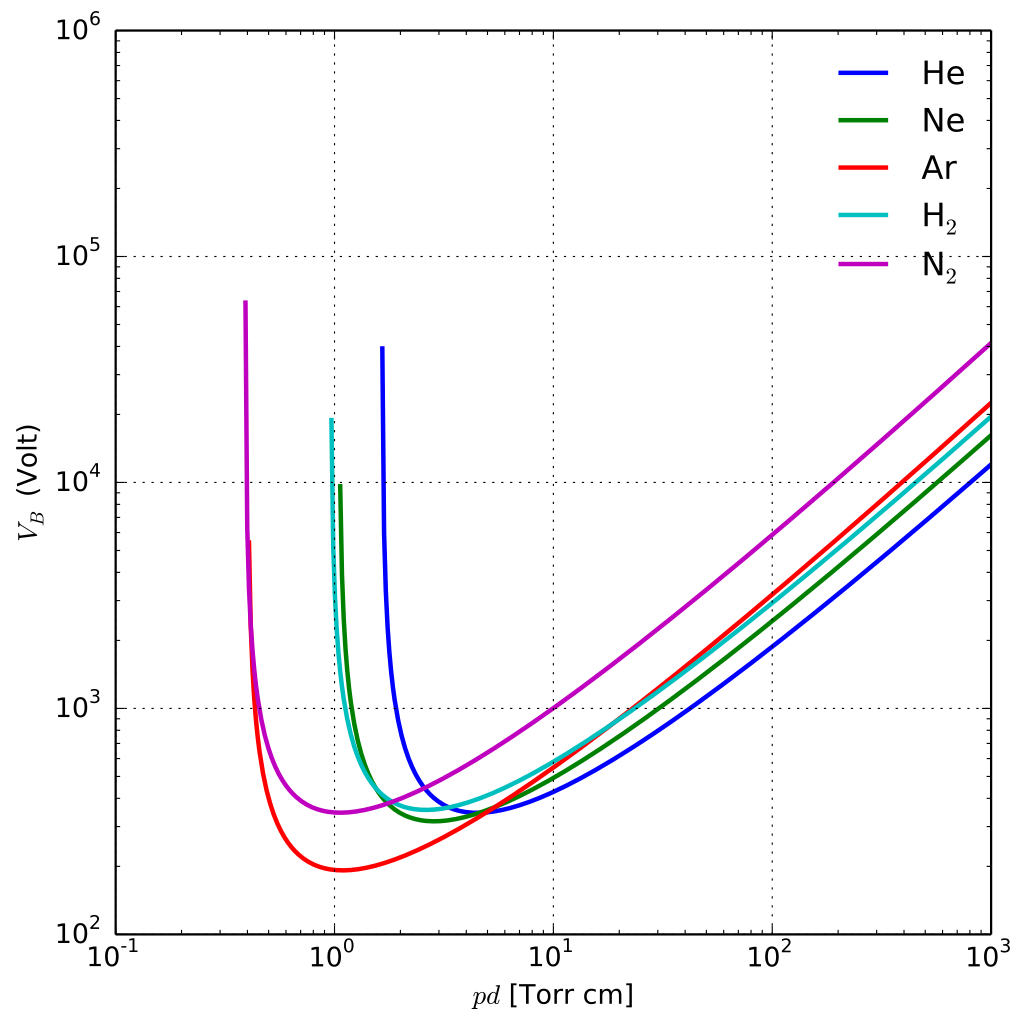
\includegraphics[width=0.75\linewidth]{chapter_2/figures/paschen_curve.png}
	\caption{Paschen curve for Helium, Neon, Argon, Hydrogen, and Nitrogen gases \cite{Lieberman2005}.}
	\label{fig:pashen_curve}
\end{figure}

\FloatBarrier

A physical explanation of Paschen's law is as follows:

\begin{itemize}
    \item \textbf{Consider the gap length remains constant}. Starting with a large pressure, the mean free path of an electron within the gas is quite short, meaning it does not have sufficient time in between collisions for it to gain enough energy to cause an ionising collision with the background gas. As the pressure is then reduced, the mean free path increases, making it easier for the electrons to gain sufficient energy to undergo ionising collisions; until a certain critical pressure (which was the aforementioned $pd$ between 1 to 10 Torr cm). Beyond this, decreasing the pressure further causes the mean free path of the electron lengthen to a point that is comparable to the gap length, therefore this decreases the likelihood of an electron colliding with a neutral gas particle and the breakdown voltage increases.
    \item \textbf{Now consider that the pressure remains constant}. When the gap length is very small, electrons are accelerated by a large electric field but are collected by the electrodes without undergoing collisions with the background gas. Increasing this gap length to a certain point gives the electrons the opportunity to collide with the background gas, producing ionising collisions. However, as the gap length continues to be increased, the strength of the electric field between the electrodes decreases, hence the electrons gain less energy between the collisions resulting in fewer ionising collisions with the background gas.
\end{itemize}

\subsection{Characteristics}

Consider a circuit as seen in figure \ref{fig:basic_circuit}. Two parallel electrodes with a DC voltage applied, and a plasma contained within a chamber. As the resistance of the variable resistor is decreased, the current through the plasma increases and one would observe three distinct discharge regions \cite{Gudmundsson2017}, shown in figure \ref{fig:dc_discharge}.

\begin{figure}[h!]
	\centering
	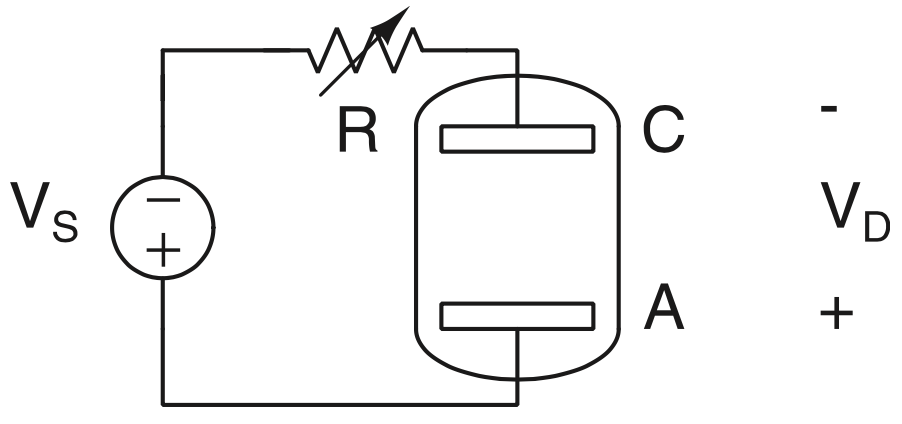
\includegraphics[width=0.45\linewidth]{chapter_2/figures/basic_circuit.png}
	\caption{Circuit diagram with a DC voltage ($V_s$) and variable resistor ($R$) to control the current through a discharge region \cite{Gudmundsson2017}.}
	\label{fig:basic_circuit}
\end{figure}

The first of these regions, is the dark discharge (or sometime referred to as the Townsend discharge) region. Initially when the voltage between the electrodes builds up, the only current through the gap is caused by pre-existing electrons, say from a previous discharge. However, this current quickly saturates (A-B in figure \ref{fig:dc_discharge}). Then, once the seed electrons gain sufficient energy, they begin ionising the background gas to produce additional electrons in a process called the \textit{Townsend avalanche} (B-D in figure \ref{fig:dc_discharge}). Once this avalanche is self-sustaining, where enough new electrons are produced to compensate for electrons lost (either to the electrodes or chamber walls), the voltage breakdown of the gas is reached (point D in figure \ref{fig:dc_discharge}).

\begin{figure}[h!]
	\centering
	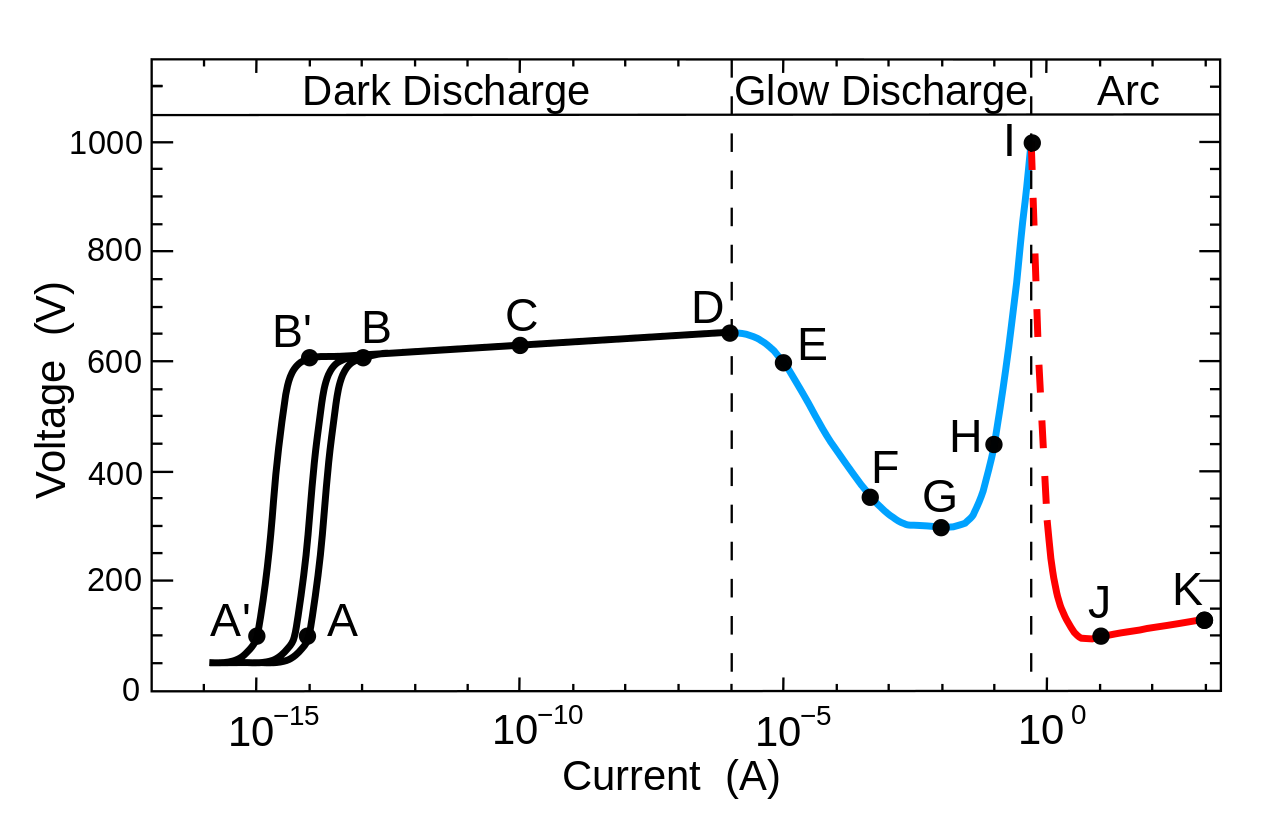
\includegraphics[width=0.8\linewidth]{chapter_2/figures/dc_discharge.png}
	\caption{Depiction of the current-voltage relationship across three discharge regions \cite{Gallo1975}.}
	\label{fig:dc_discharge}
\end{figure}

After the breakdown, the plasma is said to be in a glow discharge region. Here, the voltage across the plasma decreases since a transition from a gas to plasma state causes a decrease in resistance, implying that the ionisation process from the avalanche is more efficient (D-G in figure \ref{fig:dc_discharge}). This efficiency arises due to the high charge densities created by the plasma that perturb the applies electric field. This results in a stronger electric field near the cathode. This region of negative resistance is known as the subnormal glow. 

At first, ion bombardment on the surface of the cathode is non-uniform but as the current generated from this increases, it eventually stabilises and the distribution of the plasma (and thus the ions) across the cathode become more uniform. This is referred to as \textit{subnormal glow} and \textit{normal glow} respectively. As the current is increased further, ion bombardment across the cathode becomes saturated as it covers the entire surface of the cathode (seen from region G-I in figure \ref{fig:dc_discharge}). This is referred to as \textit{abnormal glow}, and increasing the current further causes the glow discharge to become an arc (at point I in figure \ref{fig:dc_discharge}).

In the arc discharge region, the ion bombardment onto the cathode causes the cathode to heat up to a point where electrons are generated via thermionic emission. This significantly reduces the resistance of the plasma, causing a very large drop of the voltage (seen from region I-J in figure \ref{fig:dc_discharge}). 

For the purposes of this project, the arc discharge region will be avoided because operating under arc conditions increases the electrode sputtering rate. \textit{Sputtering} is the ejection of atoms from the electrode caused by the bombardment of energetic particles. While useful for processes such as ion etching \cite{Lieberman2005}, sputtering would not be desirable as the consumption of the electrode material is something to be avoided. Sputtering has the additional downside of potentially contaminating the plasma composition as ejected atoms could end up reacting with other plasma species. 

\begin{figure}[h!]
	\centering
	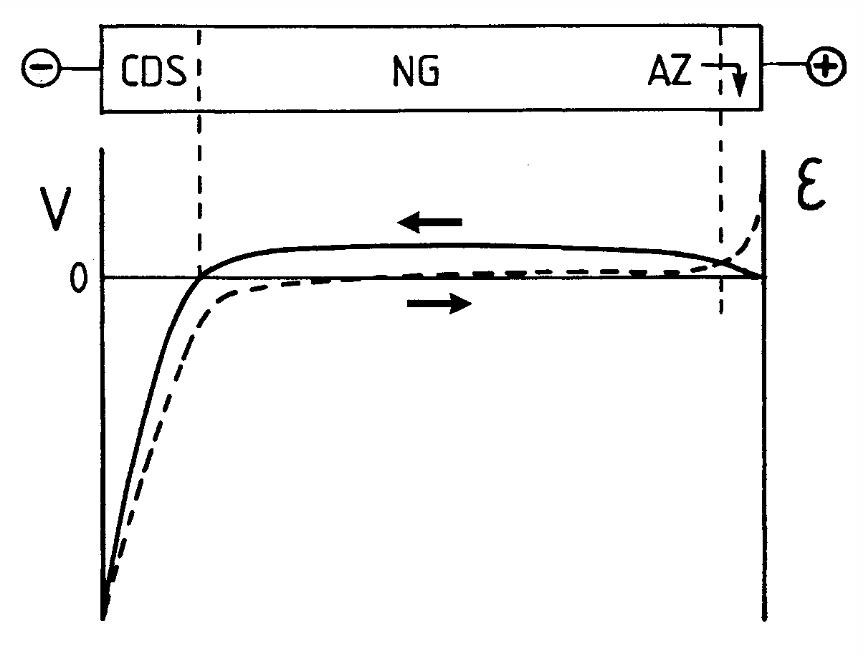
\includegraphics[width=0.7\linewidth]{chapter_2/figures/glow_discharge.png}
	\caption{Schematic highlighting the regions present in a DC glow discharge \cite{Bogaerts2002}. The cathode is on the left and the grounded anode is on the right. On the vertical axes, V is the potential and $\varepsilon$ denotes the electric field distribution. CDS is the cathode dark space, NG is the negative glow, and AZ is the anode dark space.}
	\label{fig:glow_discharge}
\end{figure}

In a glow discharge there are typical three spatial regions present. These include a \textit{cathode dark space} (CDS), a \textit{negative glow} (NG) region, and the \textit{anode dark space} (AZ) \cite{Gudmundsson2017, Bogaerts2002}. This can be observed in figure \ref{fig:glow_discharge}, that shows the potential in each region. As the distance between the electrodes is increased, additional regions may develop, however these three regions will always persist \cite{Gudmundsson2017}. The dark space regions are called \textit{sheaths} while the negative glow region is known as the \textit{bulk plasma}. Generally, the sheaths on the cathode will be much larger than that of the anode, as it corresponds to the region where electrons are being accelerated before gaining sufficient energy to cause ionising collisions. In contrast, the anode sheaths form to limit the electron current to the anode, maintaining current continuity over the discharge. Finally, the bulk plasma is the quasi-neutral region that contains the ions and electrons of the plasma.

\subsection{Discharge Sources}
\subsubsection{Parallel Plate Designs}

The simplest form of a DC plasma source is the \textit{parallel plate design}. As the name suggests, this design involves an anode and a cathode which are separated by a gap in which the plasma is formed. This is the design shown in figure \ref{fig:basic_circuit}.

An example of a device using this design can be seen in figure \ref{fig:parallel_plate_design} of a molecular emission detector by Eijkel et al\cite{Eijkel1999}. The plasma breakdown behaviour of such a design is simply governed by Paschen's law. 

\begin{figure}[h!]
	\centering
	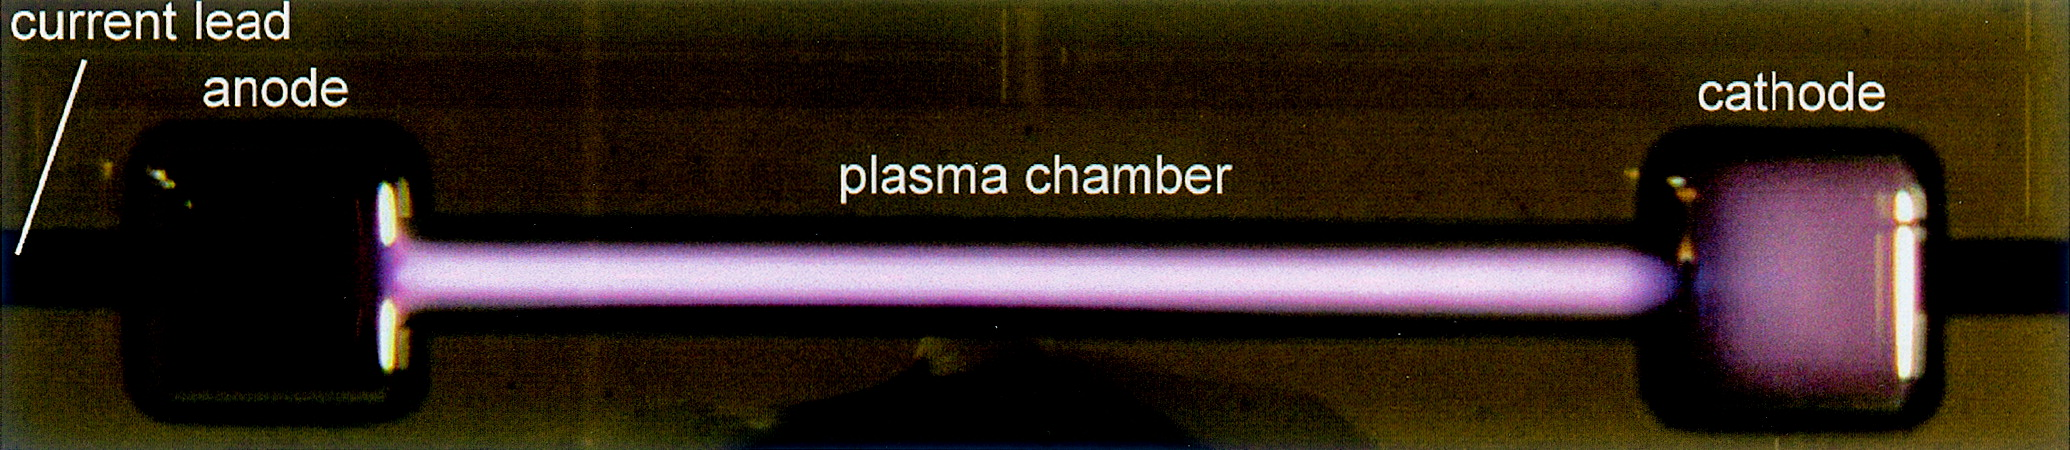
\includegraphics[width=\linewidth]{chapter_2/figures/parallel_plate.jpeg}
	\caption{A DC plasma from molecular emission detector on chip \cite{Eijkel1999}.}
	\label{fig:parallel_plate_design}
\end{figure}

Typically, parallel plate designs are favoured when simplicity and low cost are top priorities. There are some use cases such as plasma immersion ion implantation \cite{Ueda1999} and optical emission detectors \cite{Eijkel1999} where this design proves useful. However, in most scenarios this design is fundamentally flawed due to erosion of the electrode. This erosion is caused by the ion bombardment, which is a necessary process to generate secondary emission electrons; a required mechanism to sustain the plasma discharge. As such, electrode erosion limits the lifetime of a device with such a design.   

\subsubsection{Hollow Cathode Designs}

The \textit{hollow cathode design} is a commonly used alternative to the basic parallel plate geometry. Hollow cathodes are typically cylindrical in nature, where the anode remains the same but the cathode has been replaced with cup-like shape that is hollow in the centre (hence the name). An illustration of this can be seen in figure \ref{fig:hollow_cathode_design}. 

\begin{figure}[h!]
	\centering
	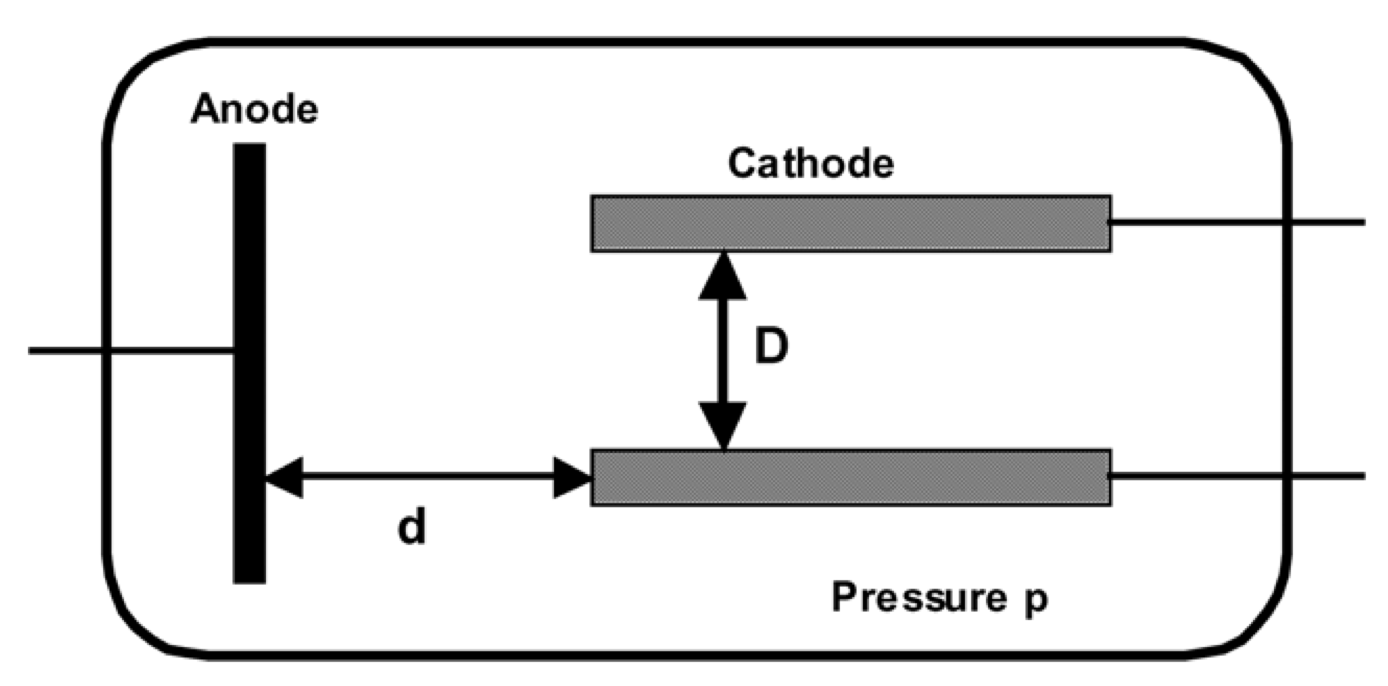
\includegraphics[width=0.6\linewidth]{chapter_2/figures/hollow_cathode_illustration.png}
	\caption{A simplified illustration of a hollow cathode design \cite{Becker2006}.}
	\label{fig:hollow_cathode_design}
\end{figure}
 
 Such a design in favourable over the parallel plate geometry because of a phenomenon known as the \textit{hollow cathode effect}. There are multiple factors that contribute to the hollow cathode effect. However, it is generally agreed upon that the primary mechanism is caused by the pendulum motion of electrons. Electrons generated via secondary-emissions from the cathode will tend to oscillate back and forth between the cathode walls, whilst slowly drifting towards the anode. This motions of electrons increases the likelihood that any given one will undergo an ionising collision with a neutral gas atom before reaching the anode \cite{Arslanbekov1998}.
 
 While the hollow cathode geometry does obey Paschen's law, an additional parameter needs to be taken into account. This new parameter is the diameter of the aperture of the cathode, shown in figure \ref{fig:hollow_cathode_design} as $D$. A general rule of thumb is that the product of the pressure and cathode aperture ($pD$) should be in the range of 1-10 Torr cm \cite{watson_gewartewski_1965}. When the $pD$ value is too large, the pendulum effect of the electrons is lost since they undergo many collisions before reaching the opposite end of the cathode. In contrast, when the $pD$ value is too small, the plasma tends to form outside the hollow cathode structure as the diameter of the aperture is comparable to the Debye length \cite{Iza2008}.
 
 Because of this, hollow cathodes have several benefits compared to their parallel plate counterparts. The most notable is that they have a lower breakdown voltage, particularly at lower gas pressures \cite{Kolobov2015, Eichhorn1993}. Additionally, they generally produce a higher current density for a given operating voltage \cite{Kolobov2015, Pillow1981}, as illustrated in figure \ref{fig:current_density_hollow_cathode}. 

\begin{figure}[h!]
	\centering
	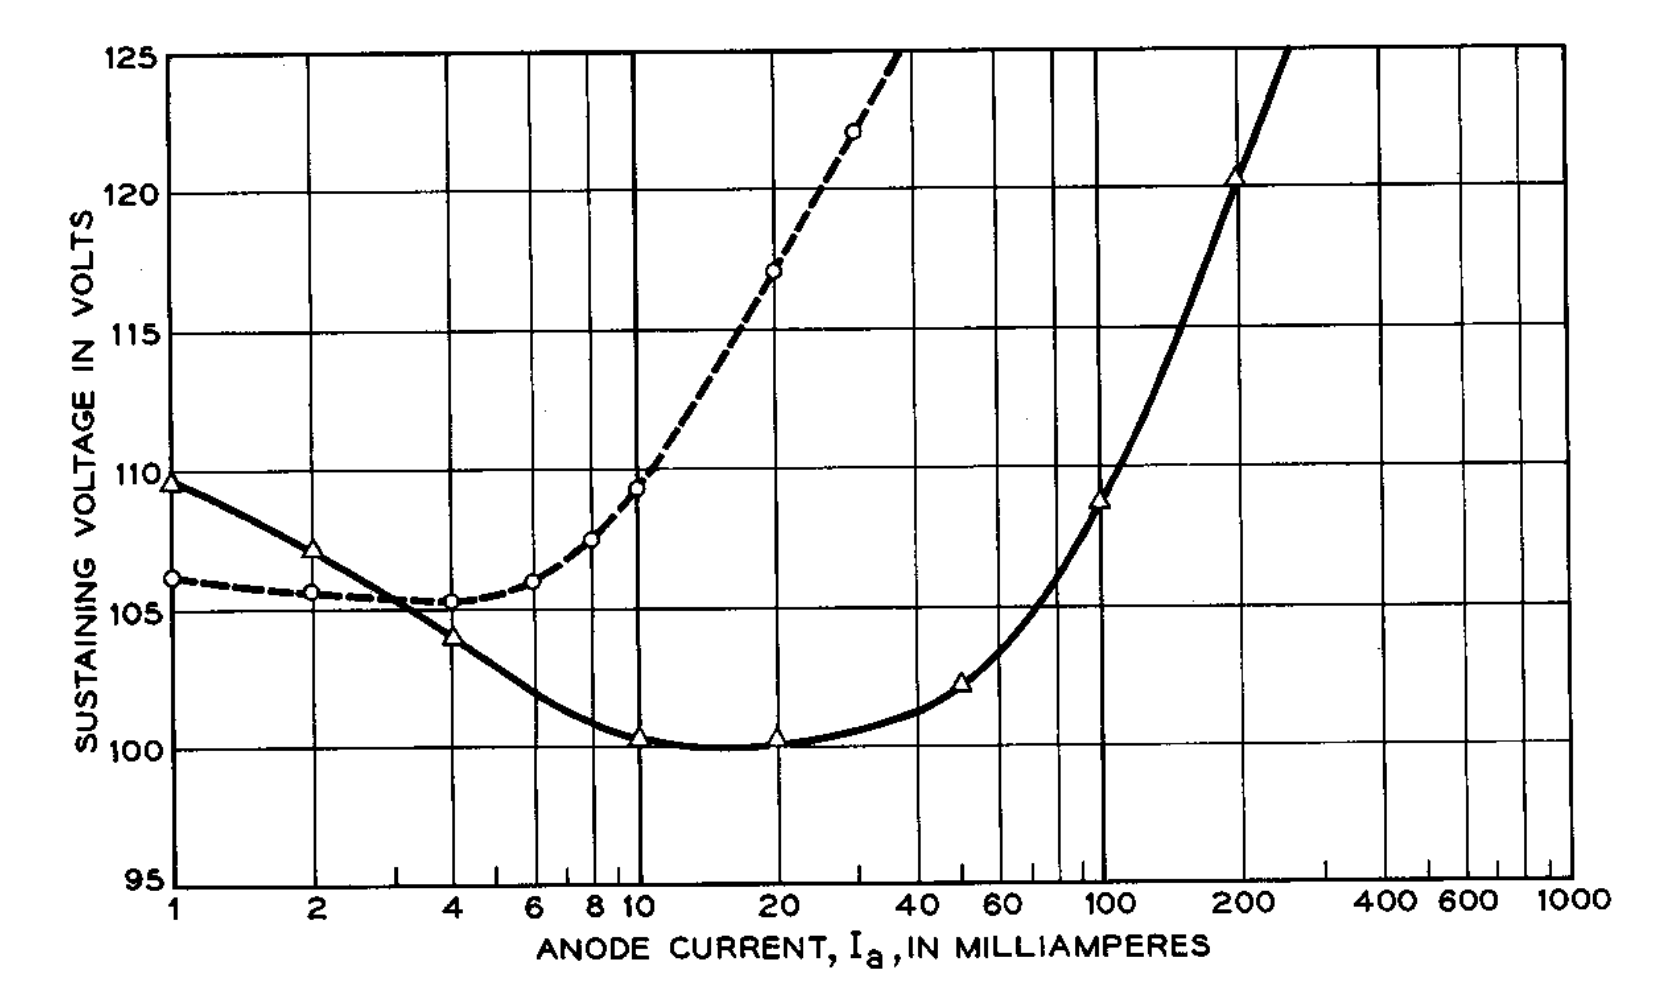
\includegraphics[width=0.95\linewidth]{chapter_2/figures/current_density_hollow_cathode.png}
	\caption{A comparison of the voltage vs current curve for a hollow cathode geometry (solid line) and a typical parallel plate geometry (dashed line)\cite{watson_gewartewski_1965}.}
	\label{fig:current_density_hollow_cathode}
\end{figure}

However, there are still several drawbacks to the hollow cathode. Despite their higher density, the vast majority of charged particle interactions are still conllisionless. This means that there is greater bombardment of the cathode, thus leading to faster erosion. Another issue is with regards to the higher current densities, meaning that a power supply that is capable of supplying the necessary current without failure is required.

Despite this, advancements and developments of the hollow cathode geometry have mitigated this by extending the life and reliability of the cathode. As such, hollow cathode designs are found in research areas such as electron beam guns \cite{Kornilov2009, YuBakeev2018} for welding and 3D printing of metals, and electrostatic propulsion \cite{Goebel2021} for spacecraft thrusters.


\section{AC Discharge}
\subsection{Breakdown and Characteristics}

If the voltage source in the circuit of figure \ref{fig:basic_circuit} were to be replaced with a low frequency AC source, the discharge behaviour would be almost identical to that of the DC discharge, provided that the half period of an AC cycle is larger than the time required for ions and electrons to move across the gap \cite{Bogaerts2002}. With such a case, the only difference compared to a DC discharge is that the electrons would move across in one direction (e.g. from left to right) in the first half period the the AC cycle, then in reverse (from right to left) in the second half period. This is because the position of the cathode and anode alternate.

However, as the frequency of the AC source is increased, typically to the region of radio or microwave frequencies, there is an asymmetry between the movement of the ions and electrons. The electrons are capable of responding to the change in the electric fields relatively quickly; however, due to the ions being significantly heavier than electrons, they have a much slower response time that is restricted by their inertia \cite{Chabert2011}.

Since the ions cannot respond to the changing electric field quick enough, they respond to the time-averaged field thus are accelerated against both electrodes cross the sheath. On the other hand, the electrons begin accelerating through the bulk plasma towards the anode during the first half period of the AC signal. Then as the direction of the electric field reverses in the second half period of the signal, the positions of the anode and cathode flip, and any electron that has not collided with the original anode (which is now the cathode), gets accelerated through the bulk plasma towards the new anode. This oscillating behaviour confines the electrons, resulting in an increased likelihood of ionising collisions with the neutral background gas. This mechanism is similar to the pendulum effect of the electrons in hollow cathode DC discharges. As the frequency of the AC source is increased, more electrons become trapped in this regime, hence it is no surprise that the breakdown voltage of the plasma decreases \cite{Chu1992}. This can be seen in figure \ref{fig:ac_breakdown}

Astute readers may notice the minimal role of the secondary emission of electrons plays in the AC discharge. This is because the ions do not need to be accelerated to high energies to induce secondary electron emissions. Thus in AC discharges, there is less erosion on the electrodes, which increases its overall lifetime. 


\begin{figure}[h!]
	\centering
	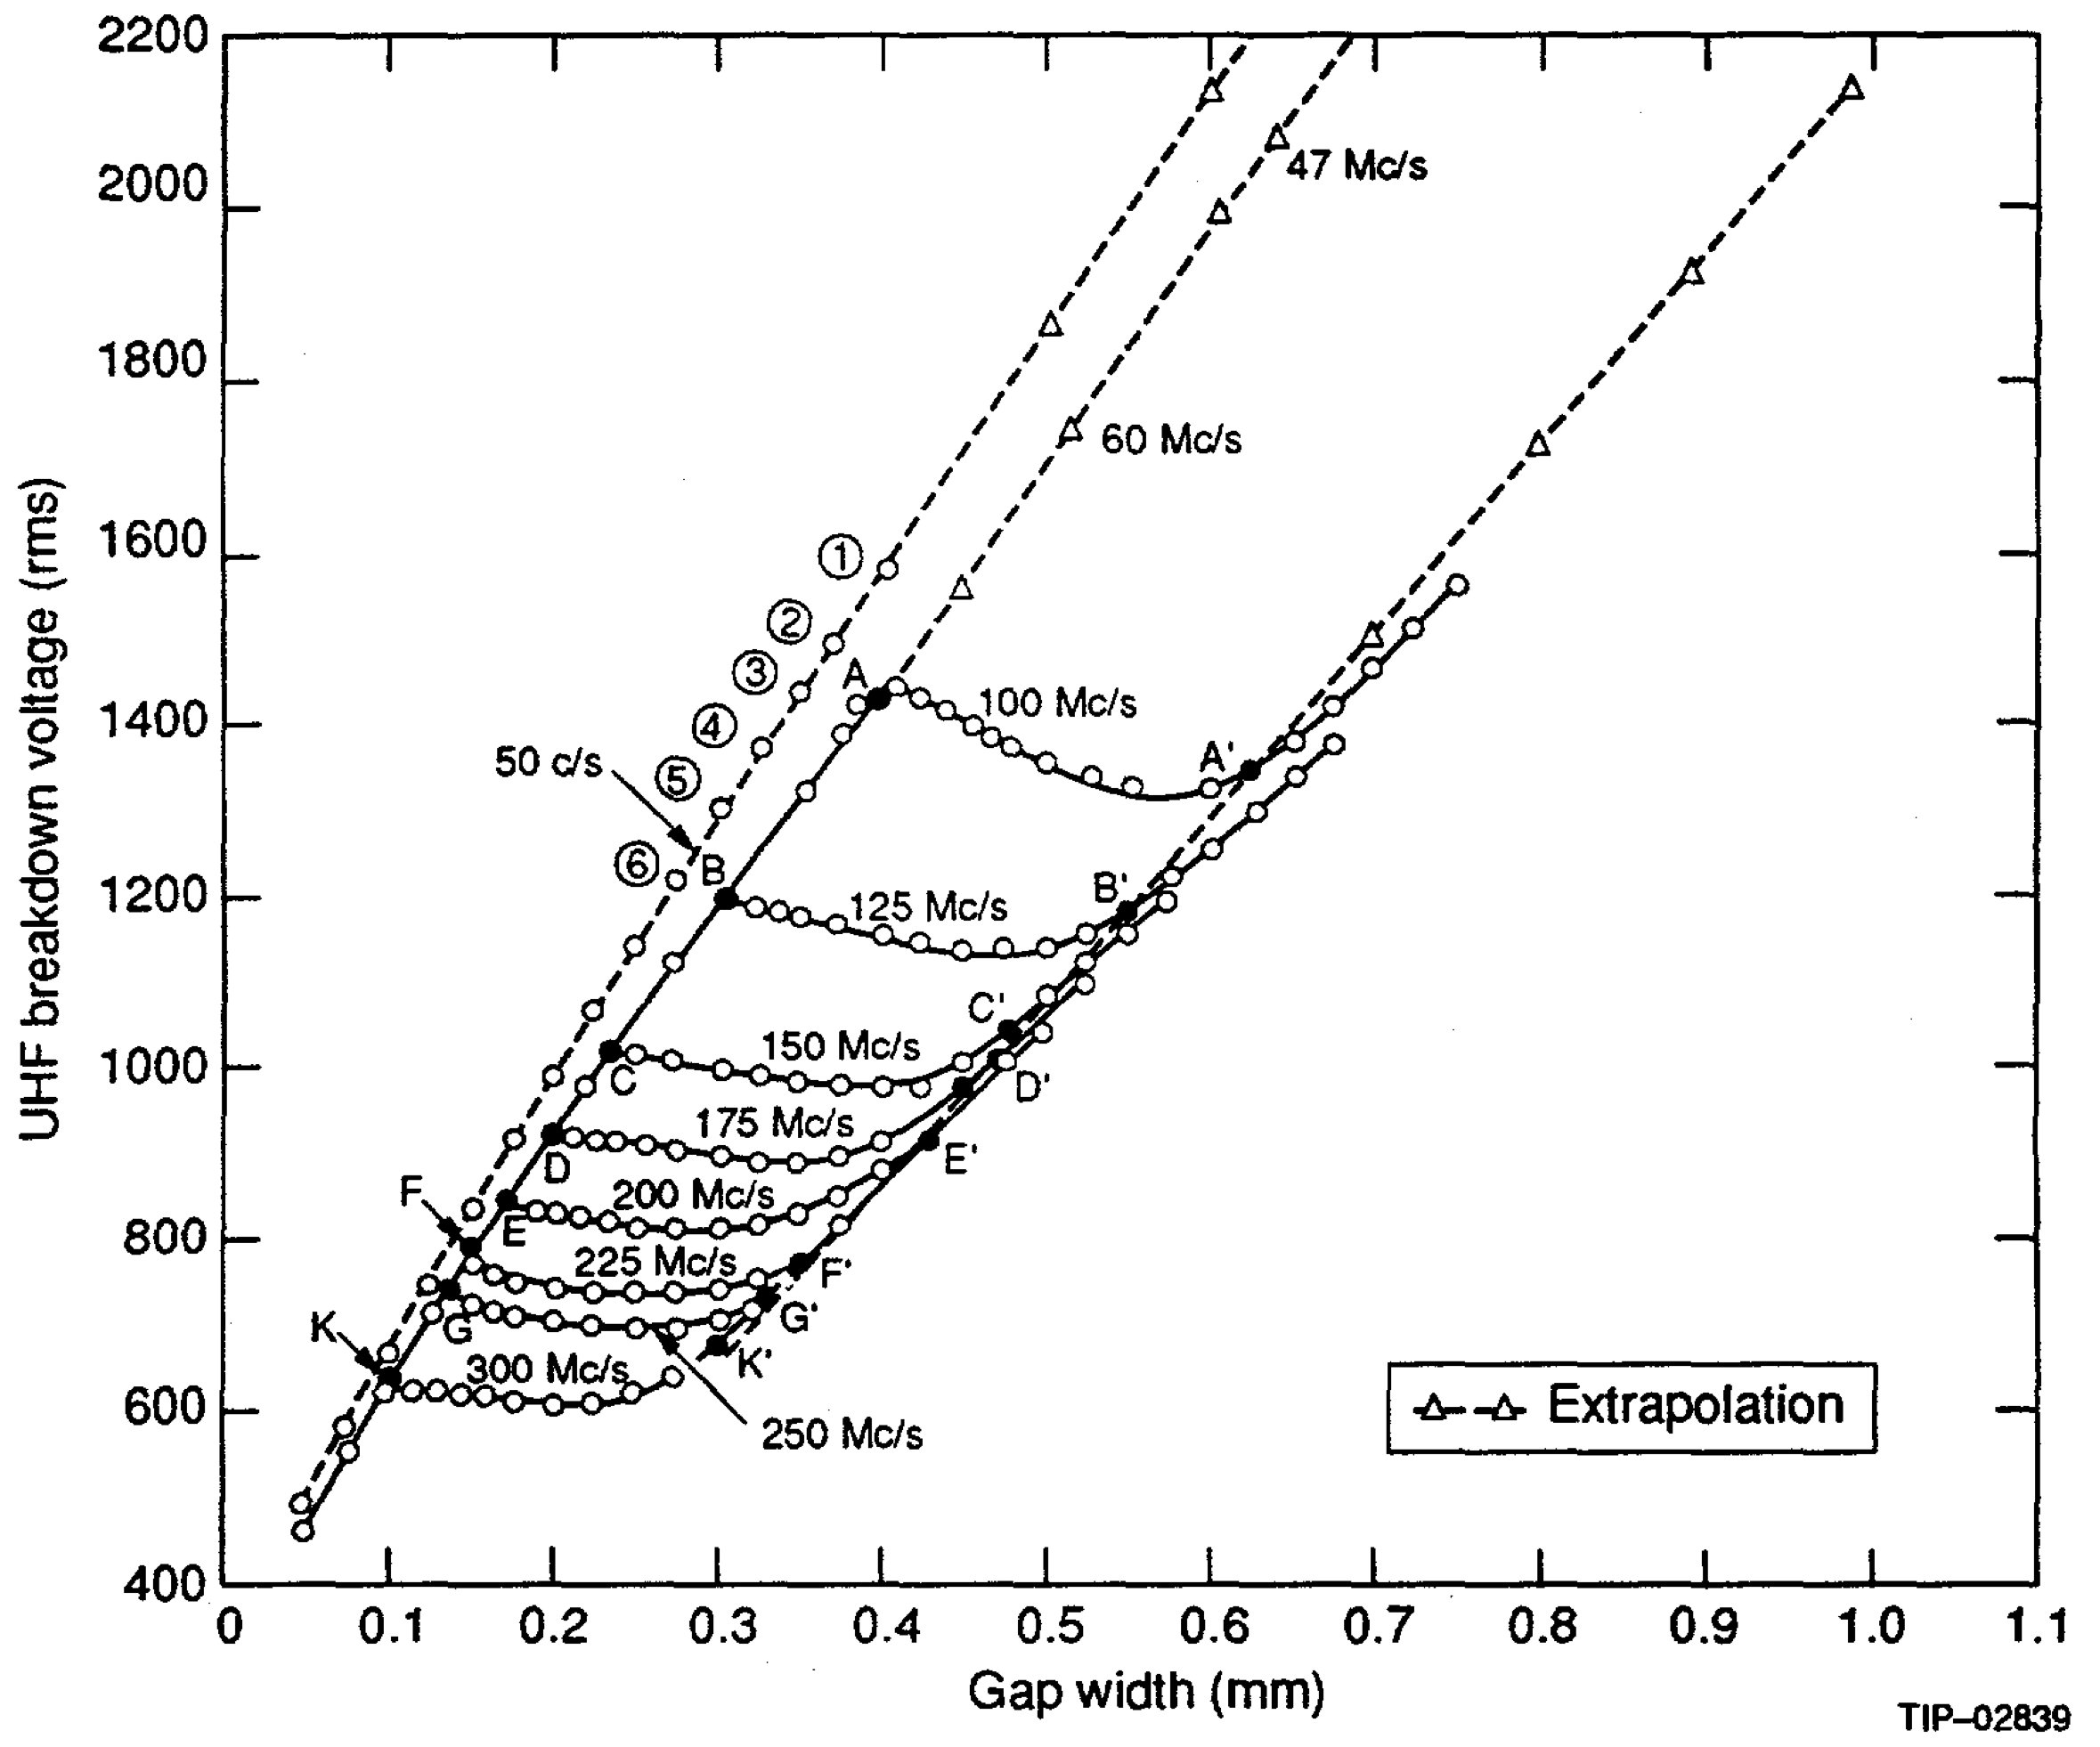
\includegraphics[width=\linewidth]{chapter_2/figures/ac_breakdown.png}
	\caption{Paschen curve for AC discharge across various frequencies \cite{Pim1949}.}
	\label{fig:ac_breakdown}
\end{figure} 


\subsection{Discharge Sources}
\subsubsection{Capacitively Coupled Plasma Designs}

\textit{Capacitively coupled plasma} (CCP) reactors are one of the simpler designs for AC discharges. The design is very similar to the parallel plate geometry seen in figure \ref{fig:basic_circuit}, however rather than a DC power supply, one or more radio frequency (RF) sources are used. It is common to see the addition of a capacitor in such circuits as well. This would typically be used to block DC currents introduced by the source or additional matching networks. This can also be deliberately introduced to add a DC bias, which in some applications (such a material processing) is used to accelerate ions against the target or substrate.

 An example of a CCP design can be seen in figure \ref{fig:CCP_reactor}. These reactors typically operate at the approved ISM frequency of 13.56 MHz, however frequencies up to 100 MHz have been used as demonstrated by Sharma et al \cite{Sharma2020}.

\begin{figure}[h!]
	\centering
	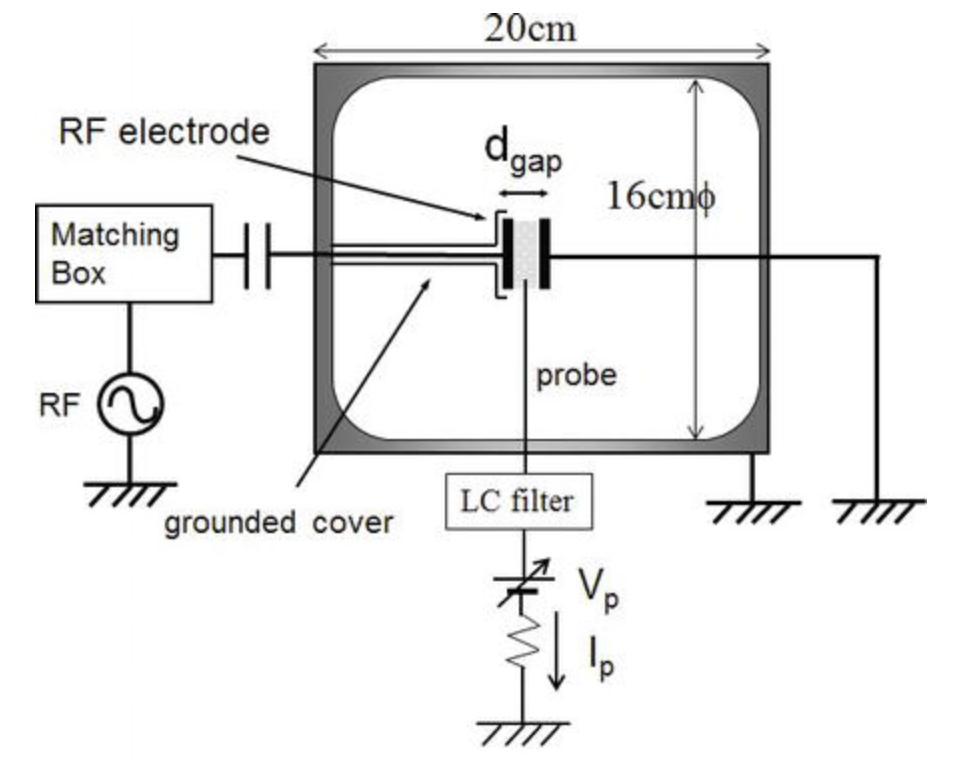
\includegraphics[width=0.6\linewidth]{chapter_2/figures/CCP_reactor.png}
	\caption{Illustration of a capacitively coupled plasma (CCP) experimental setup \cite{Ohtsu2018}.}
	\label{fig:CCP_reactor}
\end{figure} 

CCP sources are primarily used in the semiconductor industry for thin film deposition and etching. This is due to the the simple design which can be scaled fairly inexpensively. Another benefit of CCPs is that the electron temperature is fairly uniform across the entire reactor, as seen in figure \ref{fig:ccp_electron_temp}.

\begin{figure}[h!]
	\centering
	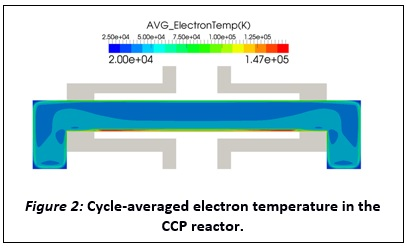
\includegraphics[width=0.6\linewidth]{chapter_2/figures/ccp_electron_temp.jpg}
	\caption{Cycle averaged electron temperature in a CCP reactor \cite{esgee_tech_2017}.}
	\label{fig:ccp_electron_temp}
\end{figure} 

However, the biggest drawback with CCP designs has to do with the limited plasma density, typically on the order of $10^{9}$ to $10^{10}$ cm$^{-3}$ \cite{Denpoh2021}. Simply increasing the input power does not translate to an increased plasma density due to energy loss by ions in the sheaths \cite{Iza2008}.

Solutions for this include dual frequency driven CCPs such as the ones by Lee and Hong \cite{Lee2021}. The idea behind such a design is that the higher frequency source controls the plasma density while the lower frequency source controls the energy of the ions bombarding the target. Other solutions including adding magnets and incorporating a hollow cathode shaped electrode to CCPs to confine the energetic electrons near the electrode \cite{Ohtsu2018}.

\subsubsection{Inductively Coupled Plasma Designs}

\begin{figure}[h!]
	\centering
	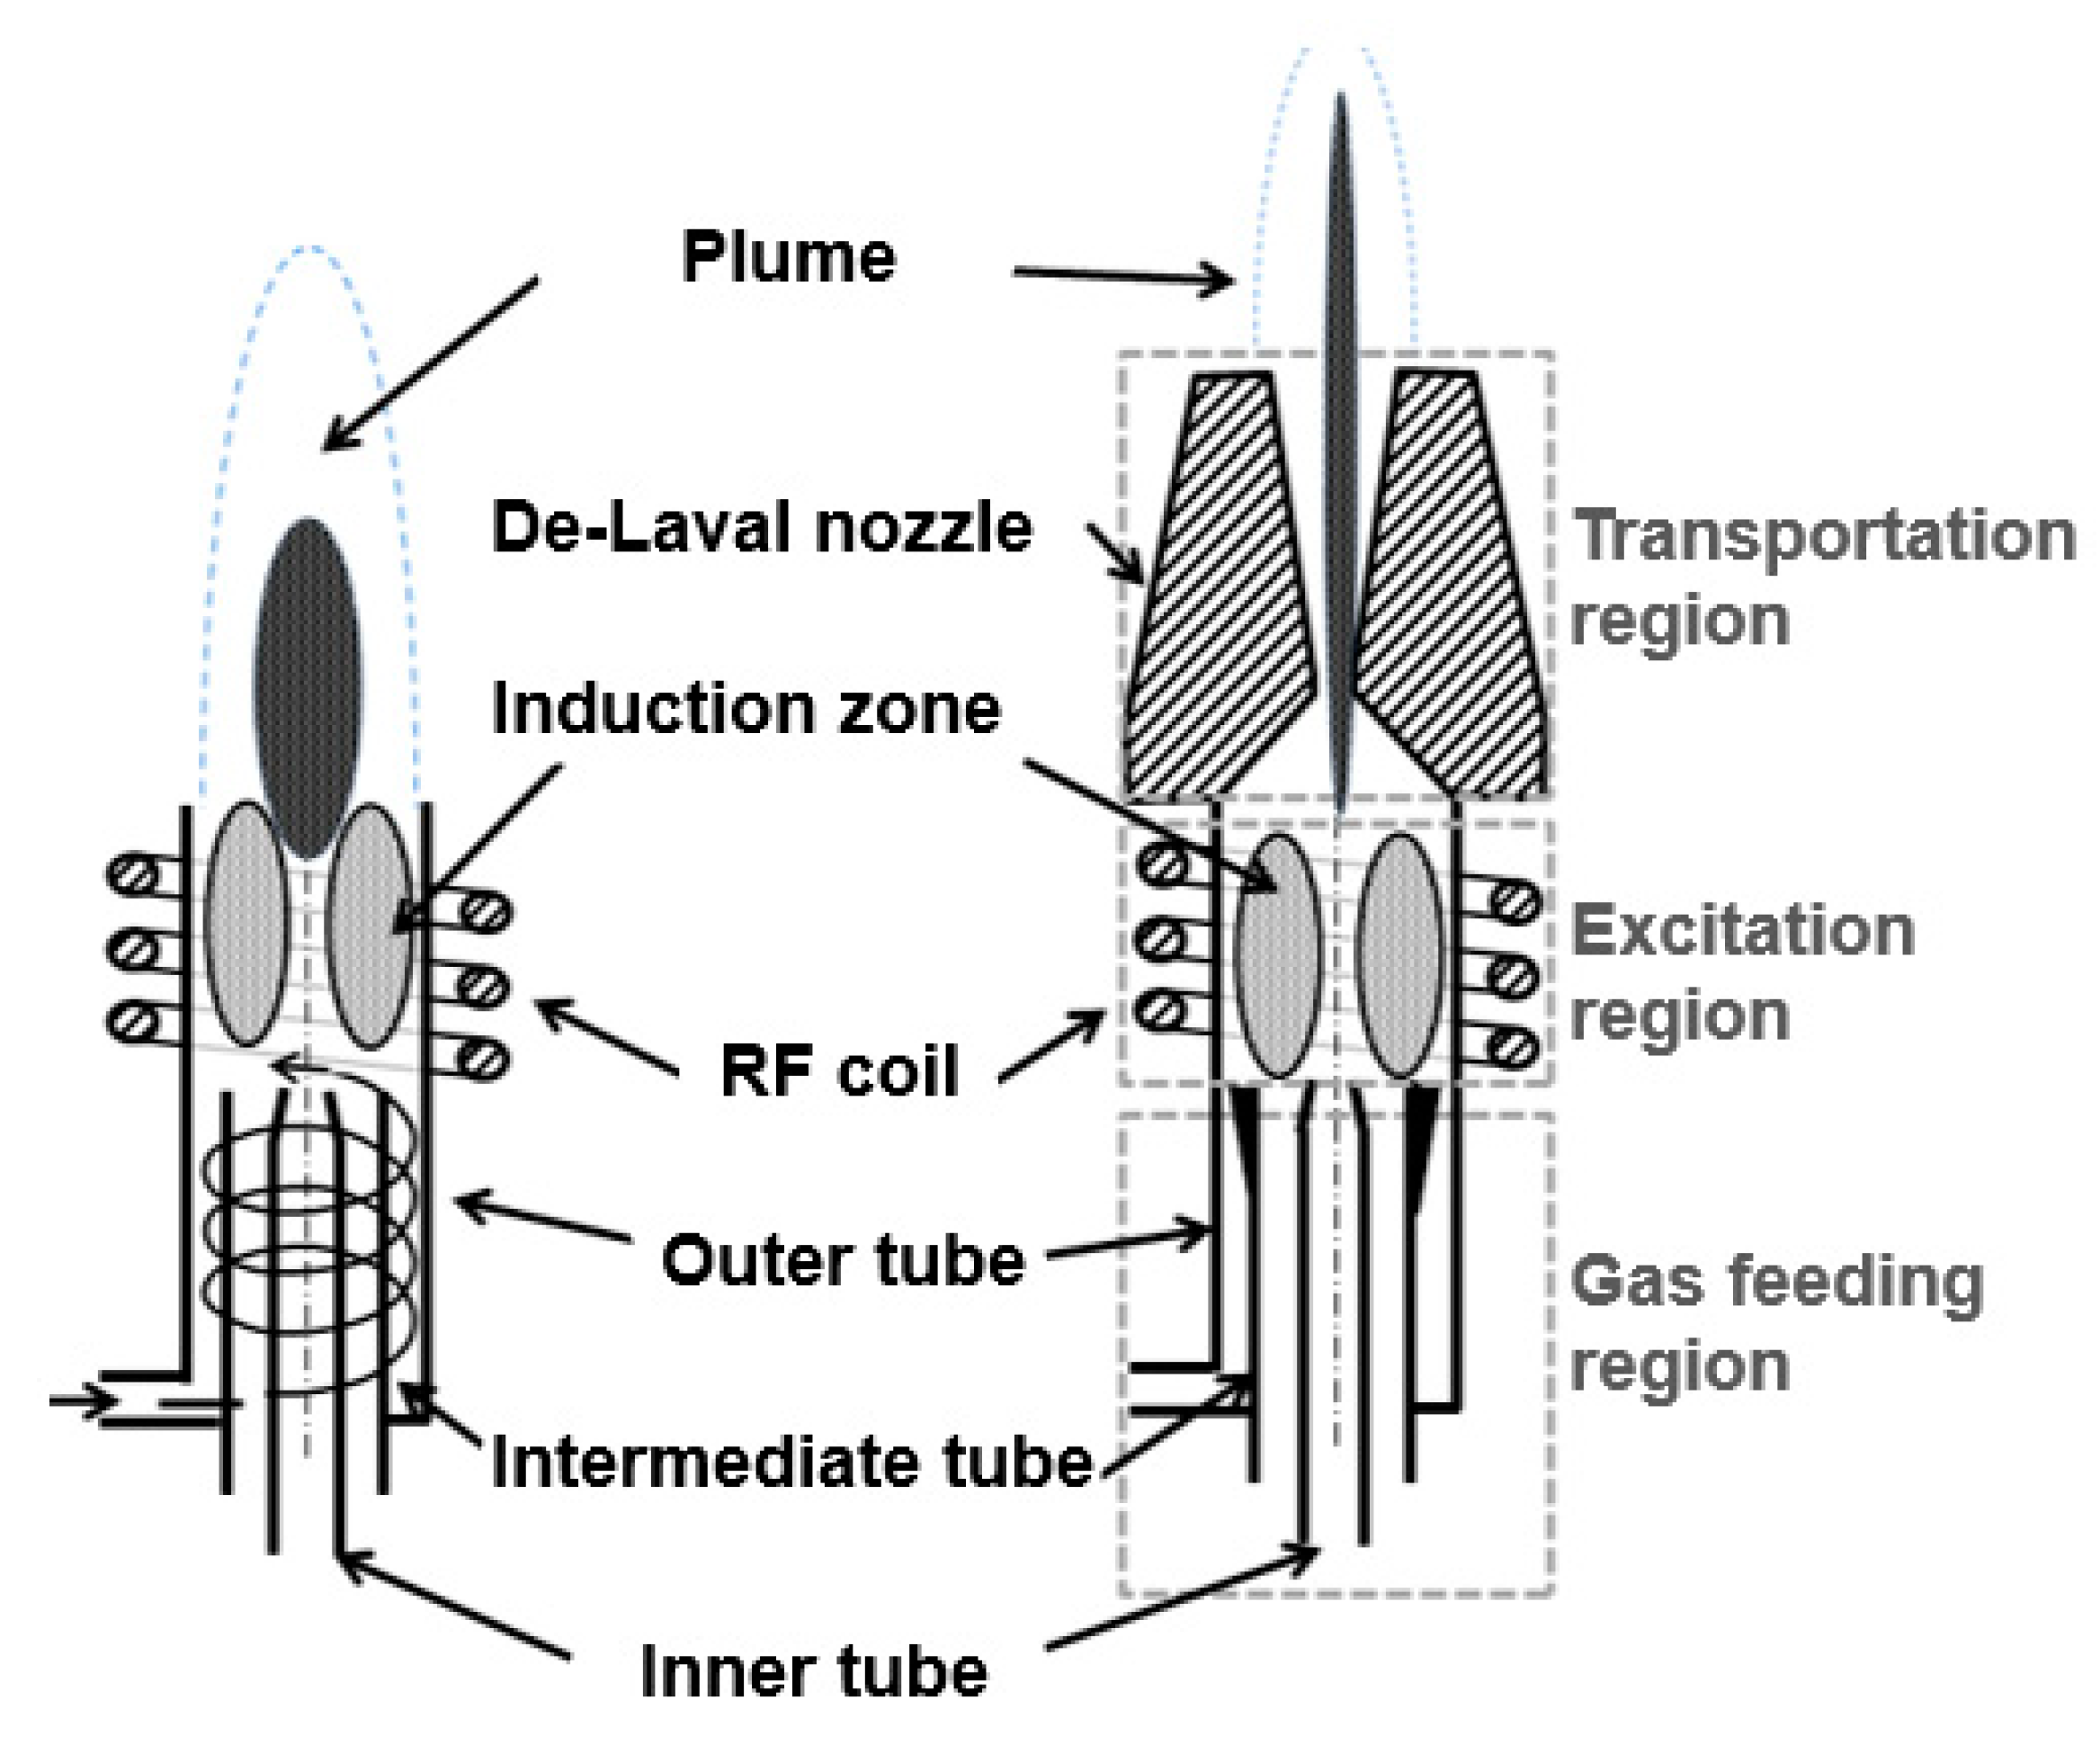
\includegraphics[width=0.75\linewidth]{chapter_2/figures/ICP_reactor.png}
	\caption{Schematic of inductively coupled plasma (ICP) torches \cite{Yu2021}.}
	\label{fig:ICP_reactor}
\end{figure} 

Another type of AC discharge source is the \textit{inductively coupled plasma} (ICP) design. The mechanism for plasma formation is different when comparing CCP and ICP designs. In CCPs, the plasma is formed by the RF voltage across a pair of parallel electrodes. However in ICPs, the plasma is generated using induction coils, relying on the phenomenon of electromagnetic induction. The RF current through the coils create a time-varying magnetic field, which in turn induces an electric field within the plasma chamber. An example of an ICP design is seen in figure \ref{fig:ICP_reactor}. 

Because the electric field in CCPs are perpendicular to the electrodes, the electrodes experience erosion due to ion bombardment. However in ICPs, the induced electric field is parallel to the walls of the reactor, thus such designs do not experience as much electrode erosion from ion bombardment or contamination of feed gas from sputtering as CCPs. Another advantage of the ICP design is that when compared to CCPs, they tend to generate a higher plasma density, especially at lower pressures. A comparison of ICP and CCP properties was done by Sakamoto et al \cite{Sakamoto2009ComparisonOP}, seen in figure \ref{fig:CCP_vs_ICP}. The results show that the electron density of ICPs were an order of magnitude greater than that of CCPs, though this did come with a drop in electron temperature. 

\begin{figure}[h!]
	\centering
	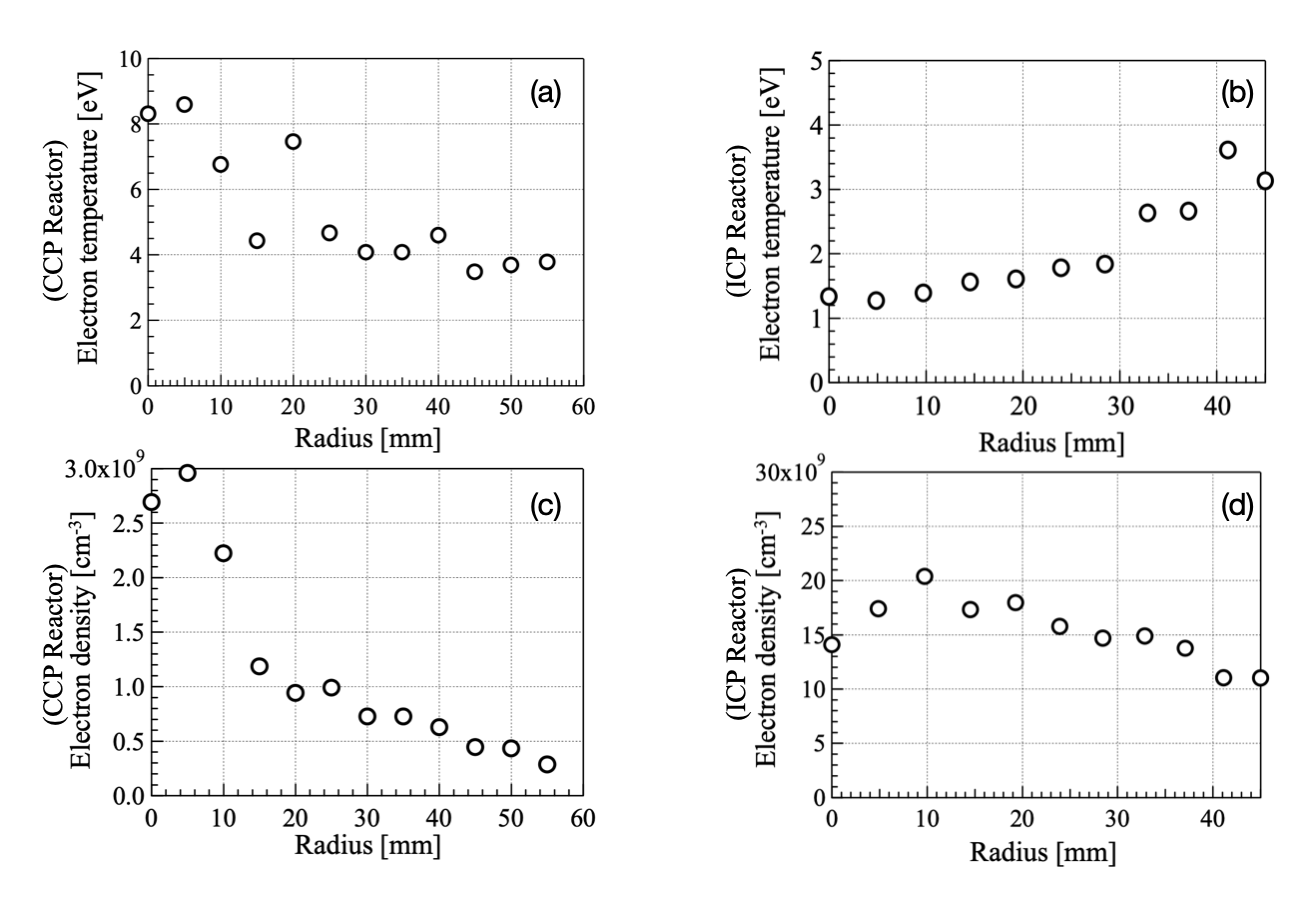
\includegraphics[width=\linewidth]{chapter_2/figures/CCP_vs_ICP_reactor.png}
	\caption{Comparison of plasma parameters between CCP and ICP reactor \cite{Sakamoto2009ComparisonOP}. The two left most graphs (a, c) are the results from a CCP reactor, while the two right most graphs (b, d) are the results of the ICP reactor. The top two graphs (a, b) show the radial distribution of electron temperatures for a CCP and ICP reactor respectively. The bottom two graphs (c, d) show the distribution of electron density for a CCP and ICP reactor respectively.}
	\label{fig:CCP_vs_ICP}
\end{figure} 


However, it has been observed that this advantage of plasma density does not necessarily continue as the size of ICPs are miniaturised. This is because the rate of decrease of inductance of the coil is much higher the coil resistance \cite{Hopwood2000}. Another downside is that ICPs are only viable at lower pressures. This is because the current in the coil required to sustain the plasma is quite high at atmospheric pressures, thus pressures between $0.1–10$ Torr are typically used \cite{Hopwood2004}.

Much like CCP reactors, ICP reactors are also used in the semiconductor industry, however they each serve different functions. For example, ICPs are used for etching of conductors whereas CCPs are used for the etching of dielectrics \cite{Kruger2020}.


\subsubsection{Dielectric Barrier Discharge Designs}

\textit{Dielectric barrier discharge} (DBD), sometimes referred to as silent discharge, is a fairly common design used on a large industrial scale. Various DBD designs can be seen in figure \ref{fig:dbd_configuartions}. Much like the parallel plate discharge, there are two electrodes, however DBD designs require the presence of at least one dielectric material in the discharge gap. 

\begin{figure}[h!]
	\centering
	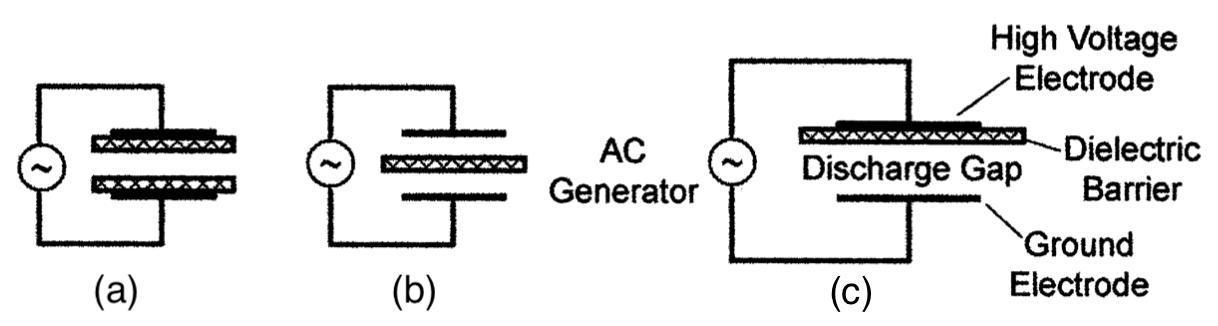
\includegraphics[width=\linewidth]{chapter_2/figures/dbd_configurations.png}
	\caption{Examples of different Dielectric Barrier Discharge (DBD) designs \cite{Kogelschatz2003}. The left most (a) and right most (c) drawings show at least one dielectric on the electrodes, while the middle (b) illustrates a dielectric in the discharge gap, but not touching the electrodes.}
	\label{fig:dbd_configuartions}
\end{figure} 

Due to the dielectric being an insulator, no conduction current can flow between the electrodes, strictly limiting DBDs to AC operation. This layer of dielectric performs two functions. The first is that it protects the electrodes from ion bombardments, preventing their erosion. Secondarily, the dielectric plays a role in limiting the average current density of the discharge, thus behaving as a ballast to prevent the transition of glow discharge to arc discharge \cite{Kogelschatz2003}.  

Most DBD devices operate in the kHz frequency range but experiments have been performed for reactors up to approximately the 10 MHz range \cite{Tingay2014}. This is because the dielectric constant of the substrate decreases at high frequencies, making it less effective at limiting the current \cite{Kogelschatz2003}.  

DBD designs were frequently used in plasma display panels, which were fairly ubiquitous in televisions until about a decade ago. Nonetheless, DBD reactors still have applications ranging from surface treatment of materials to ozone generation \cite{Brandenburg2017}.

\subsubsection{Microwave Discharge Designs}
\label{subsec:microwave_discharge}

All previous examples of AC discharges discussed so far have operated in the RF region of the electromagnetic (EM) spectrum. While there are various standard for radio bands set by agencies such as the International Telecommunication Union (ITU) or the Institute of Electrical and Electronics Engineers (IEEE), it is convention to class frequencies above 300 MHz as microwave. 

\begin{figure}[h!]
	\centering
	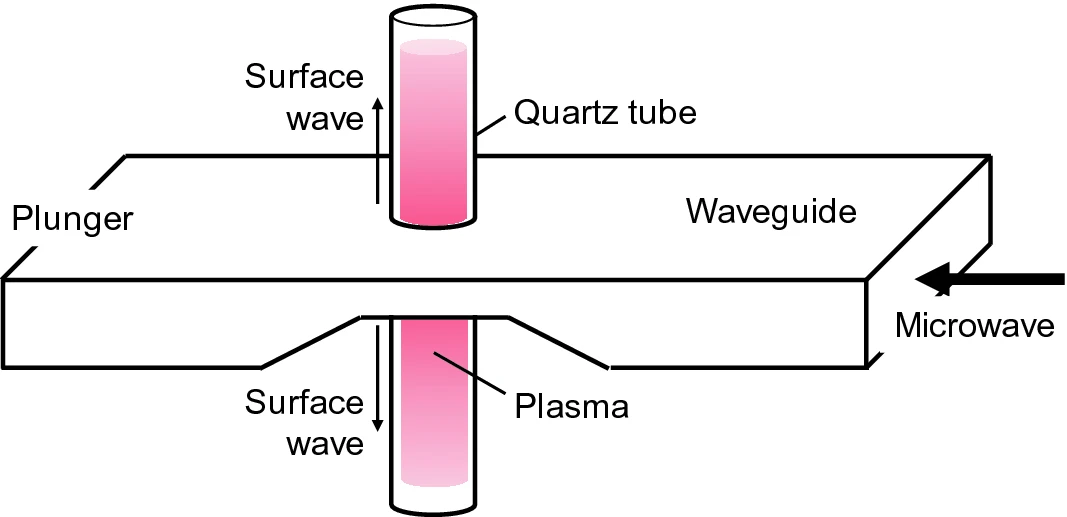
\includegraphics[width=0.6\linewidth]{chapter_2/figures/surface_wave_discharge.png}
	\caption{Schematic of a surface wave discharge plasma source \cite{Toyoda2020}.}
	\label{fig:surface_wave_discharge}
\end{figure} 

The microwave plasma sources commonly used in industry tend to be fairly large devices. One of the most common of these devices generate the plasma via \textit{surface wave discharge} where the microwaves are propagated by a wave guide \cite{Toyoda2020}, shown in figure \ref{fig:surface_wave_discharge}. The waveguides channel the microwaves to a quartz tube containing the feed gas, which when excited by the microwaves generate the plasma.  

Yet another type of microwave source is the \textit{electron cyclotron resonance} plasma reactor that combine the microwaves source with a strong magnetic field \cite{Toyoda2020}. The applied magnetic field for the electrons to move in a spiral trajectory due to the Lorentz force, and the frequency of this circular motion is called the \textit{cyclotron frequency}. Typically, the microwave frequency is fixed, thus an appropriate magnetic flux is selected to acheive the desired cyclotron frequency.

Then, a microwave frequency is selected to match this cyclotron frequency, inducing a resonance in the electrons, which in turn increase their kinetic energy. An illustration of this reactor type can be seen in figure \ref{fig:electron_cyclotron_resonance}. 

\begin{figure}[h!]
	\centering
	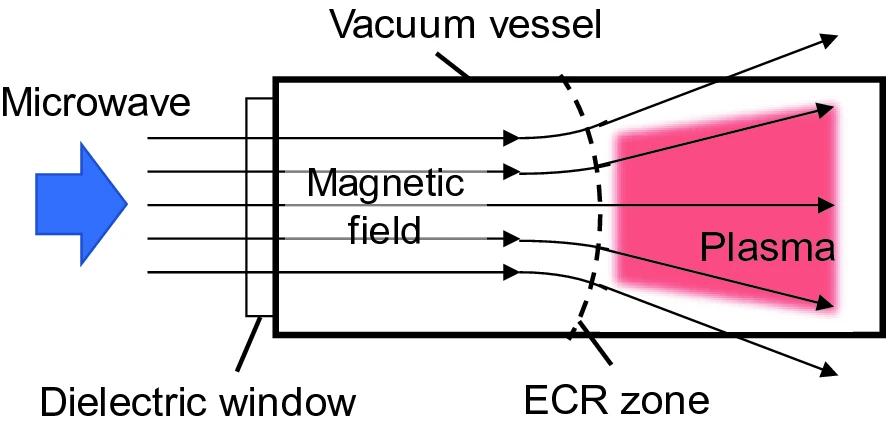
\includegraphics[width=0.55\linewidth]{chapter_2/figures/electron_cyclotron_resonance.png}
	\caption{Schematic of an electron cyclotron resonance plasma source \cite{Toyoda2020}.}
	\label{fig:electron_cyclotron_resonance}
\end{figure} 

While these larger microwave plasma reactors produce plasmas with high densities and electron energies, they tend to be quite bulky and expensive (especially in the case of electron cyclotron resonance plasma sources). Smaller microwave plasma source designs aim to bring higher plasma densities seen with the larger devices, with the benefit of reduced power consumption and potentially lower costs. These smaller sources have the added benefit of portability and the ability to integrate such sources into subsystems in close proximity to other components, with minimal electromagnetic interference.

However, miniaturising the two aforementioned designs are unfeasible. This is simply due to the fact that the size of the device determines the frequency of operation. For example a source that is approximately 1 cm would require a power supply capable at operating at around 30 GHz. Instead, these smaller plasma sources have been developed that utilise stripline and microstip technologies that are capable of generating plasma using RF and microwave frequencies \cite{Pollak2007, Iza2003}. Examples of these plasma sources can be seen in figure \ref{fig:microstrip_microwave_discharge}. 

\begin{figure}[h!]
	\centering
	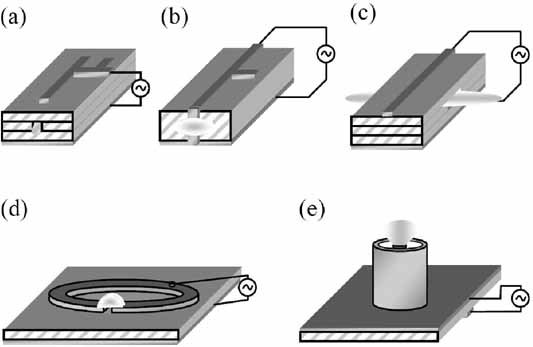
\includegraphics[width=0.8\linewidth]{chapter_2/figures/microstrip_microwave_discharge.jpg}
	\caption{Examples of different types of microstrip plasma sources \cite{Iza2008}. The top three designs (a, b, c) are linear microstrip resonators, while (d) shows a microstrip split-ring resonator, and (e) illustrates a coaxial resonator.}
	\label{fig:microstrip_microwave_discharge}
\end{figure} 

Since dimensions of the plasma formed by these microstrip sources are much smaller that the excitation wavelength, they can essentially be modelled as a CCP source. Since these microstrip sources operate at microwave frequencies, they able to take advantage of the efficiency gains obtained by operating at higher frequencies as shown in figure \ref{fig:ac_breakdown}, and have also been shown to produce higher density plasmas \cite{Surendra1998}. 

These microstrip sources have potential applications such as portable sterilisation devices \cite{Pollak2008} and chemical analysis in optical and mass spectrometry \cite{Karanassios2005}. This research intends to extend its feasibility for chemical organic synthesis.

%These microstrip sources have had many different applications such as a microplasma-based ion sensors \cite{} and atomic emission spectrometry \cite{}. This research will simply aim at extending its feasibility for chemical organic synthesis. protable device, point source sensors

